\documentclass[12pt,a4paper]{article}

% ─── Page Layout ───────────────────────────────────────────────────────────────
\usepackage[a4paper, margin=0.8in, headheight=14pt]{geometry}

% ─── Fonts (XeLaTeX) ───────────────────────────────────────────────────────────
\usepackage{fontspec}
\usepackage{unicode-math}
\setmainfont{TeX Gyre Pagella}
\setmonofont[Scale=0.88]{TeX Gyre Cursor}
\setmathfont{Latin Modern Math}

% ─── Packages ──────────────────────────────────────────────────────────────────
\usepackage{xcolor}
\usepackage{colortbl}
\usepackage{titlesec}
\usepackage{enumitem}
\usepackage{tabularx}
\usepackage{booktabs}
\usepackage{array}
\usepackage{amsmath}
\usepackage{tikz}
\usetikzlibrary{shapes.geometric, arrows.meta, positioning, calc, fit, decorations.pathreplacing, patterns}
\usepackage[american]{circuitikz}
\usepackage{tcolorbox}
\tcbuselibrary{skins, breakable}
\usepackage{hyperref}
\usepackage{fancyhdr}
\usepackage{graphicx}
\usepackage{microtype}
\hyphenpenalty=10000
\exhyphenpenalty=10000
\sloppy
\usepackage{caption}
\usepackage{setspace}
\usepackage{multirow}
\usepackage{tocloft}

% ─── Q&A helper ────────────────────────────────────────────────────────────────
\newcommand{\Q}[1]{\textbf{#1}\par\noindent\ignorespaces}

% ─── Colour Palette ────────────────────────────────────────────────────────────
\definecolor{myred}{RGB}{196,30,58}
\definecolor{mydark}{RGB}{30,30,50}
\definecolor{mygreen}{RGB}{14,120,80}
\definecolor{myteal}{RGB}{0,130,140}
\definecolor{myamber}{RGB}{180,100,0}
\definecolor{mypurple}{RGB}{100,30,160}
\definecolor{mygray}{RGB}{246,247,249}
\definecolor{mgframe}{RGB}{180,185,200}
\definecolor{watermark}{RGB}{145,150,170}
\definecolor{hdrred}{RGB}{250,232,235}
\definecolor{hdrgreen}{RGB}{220,244,233}
\definecolor{hdrteal}{RGB}{220,242,244}
\definecolor{hdramber}{RGB}{253,242,215}
\definecolor{hdrpurple}{RGB}{238,228,255}
\definecolor{hdrgray}{RGB}{238,240,245}
\definecolor{rowalt}{RGB}{250,251,253}

% ─── Section Formatting ────────────────────────────────────────────────────────
\titleformat{\section}{\large\bfseries\color{myred}}{\thesection.}{0.5em}{}[\vspace{1pt}{\color{myred}\rule{\linewidth}{0.8pt}}]
\titleformat{\subsection}{\normalsize\bfseries\color{myteal}}{\thesubsection}{0.5em}{}
\titlespacing*{\section}{0pt}{18pt}{7pt}
\titlespacing*{\subsection}{0pt}{11pt}{4pt}

% ─── Paragraph ─────────────────────────────────────────────────────────────────
\setlength{\parindent}{0pt}
\setlength{\parskip}{4pt}

% ─── TOC Styling ───────────────────────────────────────────────────────────────
\renewcommand{\cfttoctitlefont}{\large\bfseries\color{myred}}
\renewcommand{\cftaftertoctitle}{\par\noindent{\color{myred}\rule{\linewidth}{0.8pt}}}
\setlength{\cftbeforetoctitleskip}{0pt}
\setlength{\cftaftertoctitleskip}{6pt}
\renewcommand{\cftsecfont}{\normalsize\bfseries\color{mydark}}
\renewcommand{\cftsecpagefont}{\normalsize\bfseries\color{mydark}}
\renewcommand{\cftsecleader}{\cftdotfill{\cftdotsep}}
\setlength{\cftbeforesecskip}{7pt}
\renewcommand{\cftsubsecfont}{\small\color{mydark}}
\renewcommand{\cftsubsecpagefont}{\small\color{mydark}}
\setlength{\cftbeforesubsecskip}{3pt}
\setlength{\cftsubsecindent}{1.4em}

% ─── Table helpers ─────────────────────────────────────────────────────────────
\renewcommand{\arraystretch}{1.45}
\setlength{\tabcolsep}{6pt}
\arrayrulecolor{mydark}
\newcolumntype{B}[1]{>{\small\bfseries\raggedright\arraybackslash}m{#1}}
\newcolumntype{Y}{>{\small\raggedright\arraybackslash}X}
\renewcommand{\tabularxcolumn}[1]{m{#1}}

% ─── Header / Footer ───────────────────────────────────────────────────────────
\pagestyle{fancy}
\fancyhf{}
\fancyhead[L]{\small\color{myred}\textbf{PE-EC802B}\;\color{mydark}--- Industrial Automation and Control}
\fancyhead[R]{\small\color{myteal}\textbf{Module 5 Notes}}
\fancyfoot[C]{\small\color{mydark}\thepage}
\fancyfoot[R]{\small\color{watermark}\textit{\copyright\ Biraj}}
\renewcommand{\headrulewidth}{0.5pt}
\renewcommand{\footrulewidth}{0.3pt}

% ─── Hyperref ──────────────────────────────────────────────────────────────────
\hypersetup{colorlinks=true, linkcolor=myteal, urlcolor=myteal,
  pdfauthor={Biraj Sarkar}, pdftitle={PE-EC802B --- Module 5 Notes}}

% ─── tcolorbox styles ──────────────────────────────────────────────────────────
\tcbset{
  tikzbox/.style={colback=mygray, colframe=mgframe, boxrule=0.6pt, arc=4pt,
    left=8pt, right=8pt, top=6pt, bottom=6pt,
    colbacktitle=mgframe, coltitle=mydark, fonttitle=\small\bfseries},
  defbox/.style={colback=hdrgreen, colframe=mygreen, boxrule=0.8pt, arc=4pt,
    left=9pt, right=9pt, top=6pt, bottom=6pt,
    colbacktitle=mygreen, coltitle=white, fonttitle=\small\bfseries},
  formulabox/.style={colback=hdrteal, colframe=myteal, boxrule=0.8pt, arc=4pt,
    left=9pt, right=9pt, top=7pt, bottom=7pt,
    colbacktitle=myteal, coltitle=white, fonttitle=\small\bfseries},
  examplebox/.style={colback=hdramber, colframe=myamber, boxrule=0.8pt, arc=4pt,
    left=9pt, right=9pt, top=6pt, bottom=6pt,
    colbacktitle=myamber, coltitle=white, fonttitle=\small\bfseries},
  masonbox/.style={colback=hdrpurple, colframe=mypurple, boxrule=0.8pt, arc=4pt,
    left=9pt, right=9pt, top=6pt, bottom=6pt,
    colbacktitle=mypurple, coltitle=white, fonttitle=\small\bfseries},
  exambox/.style={colback=hdrpurple, colframe=mypurple, boxrule=1pt, arc=5pt,
    left=10pt, right=10pt, top=8pt, bottom=8pt,
    colbacktitle=mypurple, coltitle=white, fonttitle=\bfseries,
    breakable, title after break={\textbf{Frequently Asked / Viva Questions (contd.)}}}
}
\tcbset{breakable}

% ─── TikZ styles ───────────────────────────────────────────────────────────────
\tikzset{
  block/.style={rectangle, draw=myteal, fill=hdrteal,
    text width=2.4cm, align=center, minimum height=0.95cm,
    font=\small, rounded corners=3pt, line width=0.7pt},
  redblock/.style={rectangle, draw=myred, fill=hdrred,
    text width=2.4cm, align=center, minimum height=0.95cm,
    font=\small, rounded corners=3pt, line width=0.7pt},
  sumjunc/.style={circle, draw=myamber, fill=hdramber,
    minimum size=0.62cm, font=\small, line width=0.8pt},
  arrow/.style={-Stealth, thick, color=mydark},
  line/.style={thick, color=mydark}
}

% ═══════════════════════════════════════════════════════════════════════════════
\begin{document}
% ═══════════════════════════════════════════════════════════════════════════════

\begin{center}
  {\LARGE\bfseries\color{myred} PE-EC802B --- Industrial Automation and Control}\\[5pt]
  {\normalsize\color{mydark} Semester VIII \quad$\bullet$\quad 3L:0T:0P \quad$\bullet$\quad 3 Credits}\\[3pt]
  {\normalsize\color{myteal}\textbf{Module 5 Exam Notes}}\\[3pt]
  {\small\color{mydark} CGEC \;$|$\; B.Tech ECE (2023--27) \;$|$\; \textit{Biraj Sarkar}}
\end{center}
\vspace{2pt}
\noindent{\color{myred}\rule{\linewidth}{1.5pt}}
\vspace{2pt}

\hypersetup{linkcolor=mydark}
\tableofcontents
\hypersetup{linkcolor=myteal}
\newpage

% ===============================================================================
\section{Distributed Control Systems (DCS) \& SCADA}
% ===============================================================================

\subsection{1. Distributed Control Systems (DCS)}
A \textbf{DCS} is a control system for a manufacturing plant or process wherein controller functions are distributed throughout the system rather than centralized in a single controller. This distribution provides high scalability, reliability, and ease of loop tuning.

\textbf{1. Hierarchical Architecture (ISA-95 Levels):}
\begin{itemize}[leftmargin=*, itemsep=2.5pt]
  \item \textbf{Level 0 (Field Level):} Sensors (temperature, pressure), actuators, and control valves that interface directly with the process.
  \item \textbf{Level 1 (Direct Control Level):} Distributed controllers (microprocessor-based) that execute fast local PID algorithms and output direct control signals.
  \item \textbf{Level 2 (Supervisory Control Level):} Operators HMIs, supervisory computers, and engineering workstations that manage setpoints, monitor trends, and record alarm logs.
  \item \textbf{Level 3 (Manufacturing Operations Level):} Manufacturing Execution Systems (MES) for production scheduling, quality tracking, and inventory management.
  \item \textbf{Level 4 (Business Planning Level):} Enterprise Resource Planning (ERP) servers for corporate and financial planning.
\end{itemize}

\textbf{2. Functional Requirements:}
A DCS must support the following core functions:
\begin{itemize}[leftmargin=*, itemsep=2pt]
  \item \textbf{Data Acquisition:} Scanning analog and digital inputs from field devices.
  \item \textbf{Continuous Loop Control:} Executing PID loops with cycle times down to $10\,$ms.
  \item \textbf{Alarm Management:} Identifying and sorting process deviations (Hi/Hi-Hi alarms).
  \item \textbf{Historical Archiving:} Long-term logging of variables for audit and safety.
\end{itemize}

\textbf{3. DCS Advantages:}
\begin{itemize}[leftmargin=*, itemsep=2pt]
  \item \textbf{System Reliability (No Single Point of Failure):} Control tasks are isolated. If one controller fails, only its local loops are affected, while the rest of the plant continues running.
  \item \textbf{Redundancy:} High-availability hardware, including redundant processors in hot-standby mode (bumpless transfer under $< 50\,$ms), redundant power grids, and dual-ring communication networks.
  \item \textbf{Modularity and Scalability:} Easier to expand by adding new I/O cards or controllers.
\end{itemize}

\textbf{4. Communication for Distributed Control:}
DCS controllers communicate via deterministic, high-speed industrial networks to guarantee loop synchronization:
\begin{itemize}[leftmargin=*, itemsep=2pt]
  \item \textbf{Fieldbus/Profibus:} For connecting Level 0 field instruments to Level 1 controllers.
  \item \textbf{Industrial Ethernet:} For high-bandwidth communication between Level 1 controllers and Level 2 supervisory HMIs, often configured in a redundant physical ring topology.
\end{itemize}

\textbf{5. DCS Application Examples:}
DCS is ideal for complex, continuous, multi-loop processes:
\begin{itemize}[leftmargin=*, itemsep=2pt]
  \item \textbf{Chemical and Petrochemical Plants:} Monitoring and controlling thousands of interacting pressure, flow, and temperature loops in distillation columns and reactors.
  \item \textbf{Power Generation Plants:} Boiler combustion control, steam turbine regulation, and cooling water loop orchestration.
\end{itemize}

\subsection{2. SCADA Systems}
\textbf{SCADA} (Supervisory Control and Data Acquisition) systems are used to monitor and control large-scale, geographically distributed utility networks (electrical grids, oil/gas pipelines, water networks). Unlike a DCS, SCADA focuses on data collection and supervisory-level control over long distances, leaving local loop execution to local controllers.

\begin{tcolorbox}[tikzbox, title={Geographically Distributed SCADA System Architecture}]
\centering
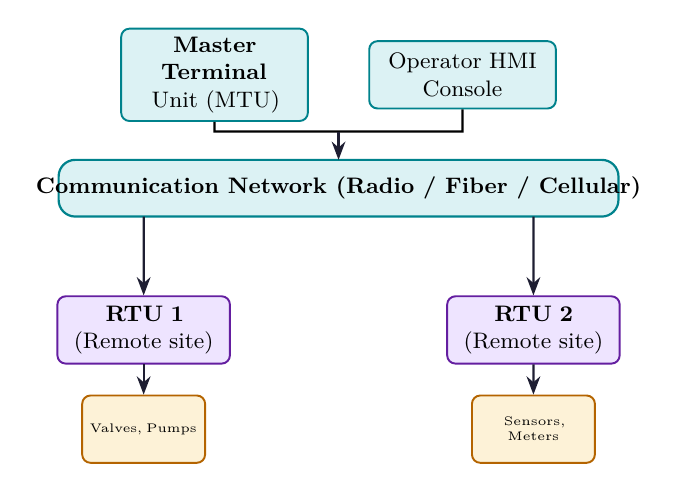
\begin{tikzpicture}[scale=0.9, transform shape]
  % MTU
  \node[block, text width=2.4cm, minimum height=1.2cm] (mtu) at (0, 1.8) {\textbf{Master Terminal}\\Unit (MTU)};
  \node[block, text width=2.4cm] (hmi) at (3.5, 1.8) {Operator HMI\\Console};

  % Communication Cloud
  \draw[thick, draw=myteal, fill=hdrteal, rounded corners=6pt] (-2.2, -0.2) rectangle (5.7, 0.6);
  \node[font=\small\bfseries] at (1.75, 0.2) {Communication Network (Radio / Fiber / Cellular)};

  % RTU 1
  \node[block, text width=2.2cm, draw=mypurple, fill=hdrpurple] (rtu1) at (-1.0, -1.8) {\textbf{RTU 1}\\(Remote site)};
  % RTU 2
  \node[block, text width=2.2cm, draw=mypurple, fill=hdrpurple] (rtu2) at (4.5, -1.8) {\textbf{RTU 2}\\(Remote site)};

  % Field devices
  \node[block, text width=1.5cm, draw=myamber, fill=hdramber, font=\tiny] (dev1) at (-1.0, -3.2) {Valves, Pumps};
  \node[block, text width=1.5cm, draw=myamber, fill=hdramber, font=\tiny] (dev2) at (4.5, -3.2) {Sensors, Meters};

  % Connections
  \draw[thick] (mtu.south) -- (0, 1.0) -- (3.5, 1.0) -- (hmi.south);
  \draw[arrow] (1.75, 1.0) -- (1.75, 0.6);
  
  \draw[arrow] (-1.0, -0.2) -- (rtu1.north);
  \draw[arrow] (4.5, -0.2) -- (rtu2.north);
  
  \draw[arrow] (rtu1) -- (dev1);
  \draw[arrow] (rtu2) -- (dev2);
\end{tikzpicture}
\end{tcolorbox}

\textbf{1. Core Components \& Architecture:}
\begin{itemize}[leftmargin=*, itemsep=2.5pt]
  \item \textbf{MTU (Master Terminal Unit):} The central host server located at the control center. It polls remote stations, archives telemetry data, updates the HMI database, and transmits supervisory commands.
  \item \textbf{RTU (Remote Terminal Unit):} Microprocessor units deployed at remote field sites. They interface with local sensors and actuators, convert signals to digital data, and communicate with the MTU.
  \item \textbf{HMI (Human Machine Interface):} Visual display stations in the control room showing real-time trends, piping \& instrumentation diagrams (P\&ID), and active system alarms.
\end{itemize}

\textbf{2. SCADA Communication \& Telemetry:}
Because SCADA nodes are miles apart, communication is often non-deterministic, using varied media:
\begin{itemize}[leftmargin=*, itemsep=2.5pt]
  \item \textbf{Media:} Radio telemetry, cellular networks (LTE/5G), satellite links, and fiber optics.
  \item \textbf{Polling vs. Event-Driven (Report-by-Exception):} To conserve network bandwidth, SCADA RTUs do not transmit data continuously. In \textbf{Report-by-Exception (RBE)}, the RTU only transmits data if the measured variable changes beyond a preset deadband or if an alarm is triggered.
  \item \textbf{Protocols:} Modbus (legacy, serial/TCP), DNP3 (Distributed Network Protocol, optimized for utilities with time-stamping), and OPC UA (Open Platform Communications Unified Architecture, secure, platform-independent).
\end{itemize}

\textbf{3. SCADA Application Examples:}
SCADA is suited for geographically dispersed networks with low control-loop speeds:
\begin{itemize}[leftmargin=*, itemsep=2pt]
  \item \textbf{Electrical Power Transmission Grids:} Monitoring sub-station switchgears, busbar voltages, and power flow over thousands of square miles.
  \item \textbf{Oil and Gas Pipelines:} Tracking pressure profiles, flow rates, and leak detection across transcontinental pipeline routes, automatically closing remote valves during pressure drops.
  \item \textbf{Water Distribution Systems:} Monitoring water reservoir levels, pipe pressures, and controlling pumping stations across municipal regions.
\end{itemize}


% ===============================================================================
\section{Advanced Industrial Control Techniques}
% ===============================================================================

\subsection{1. Cascade Control}
Cascade control utilizes two nested feedback loops (an inner fast loop and an outer slow loop) to improve disturbance rejection.

\begin{tcolorbox}[tikzbox, title={Cascade Control System Block Diagram}]
\centering
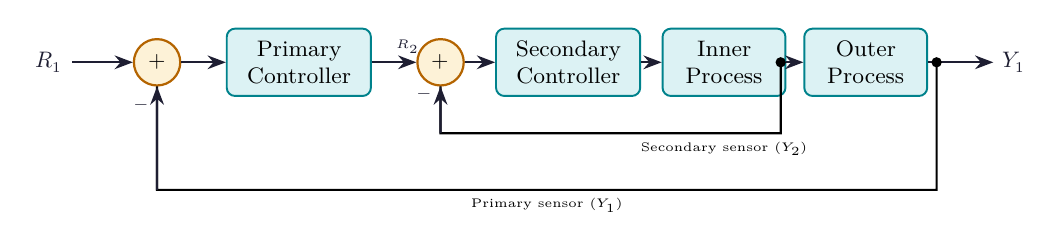
\begin{tikzpicture}[scale=0.9, transform shape]
  % Summer 1 (Outer)
  \node[sumjunc] (sum1) at (-2.0, 0) {$+$};
  \node[block, text width=1.8cm] (ctrl1) at (0, 0) {Primary\\Controller};
  
  % Summer 2 (Inner)
  \node[sumjunc] (sum2) at (2.0, 0) {$+$};
  \node[block, text width=1.8cm] (ctrl2) at (3.8, 0) {Secondary\\Controller};
  
  \node[block, text width=1.5cm] (p1) at (6.0, 0) {Inner\\Process};
  \node[block, text width=1.5cm] (p2) at (8.0, 0) {Outer\\Process};

  % Paths
  \draw[arrow] (-3.2,0) node[left, font=\small] {$R_1$} -- (sum1);
  \draw[arrow] (sum1) -- (ctrl1);
  \draw[arrow] (ctrl1) -- (sum2) node[above, pos=0.8, font=\tiny] {$R_2$};
  \draw[arrow] (sum2) -- (ctrl2);
  \draw[arrow] (ctrl2) -- (p1);
  \draw[arrow] (p1) -- (p2);
  \draw[arrow] (p2) -- (9.8, 0) node[right, font=\small] {$Y_1$};

  % Inner feedback
  \draw[thick] (6.8, 0) to[short, *-] (6.8, -1.0) -| (sum2);
  \draw[arrow] (2.0, -1.0) -- (sum2) node[left, pos=0.8, font=\scriptsize] {$-$};
  \node[below, font=\tiny] at (6.0, -1.0) {Secondary sensor ($Y_2$)};

  % Outer feedback
  \draw[thick] (9.0, 0) to[short, *-] (9.0, -1.8) -| (sum1);
  \draw[arrow] (-2.0, -1.8) -- (sum1) node[left, pos=0.8, font=\scriptsize] {$-$};
  \node[below, font=\tiny] at (3.5, -1.8) {Primary sensor ($Y_1$)};
\end{tikzpicture}
\end{tcolorbox}

\begin{itemize}[leftmargin=*, itemsep=2.5pt]
  \item \textbf{Working:} The outer primary controller computes the setpoint $R_2$ for the inner secondary loop. 
  \item \textbf{Advantage:} Disturbances originating inside the inner loop (e.g. pressure fluctuations in a fuel valve feed) are corrected instantly by the secondary controller before they can affect the primary process output $Y_1$.
\end{itemize}

\subsection{2. Feedforward Control}
Feedforward control measures disturbances ($D$) directly and compensates for them *before* they can affect the process variable ($Y$).

\begin{tcolorbox}[tikzbox, title={Combined Feedforward-Feedback Control System}]
\centering
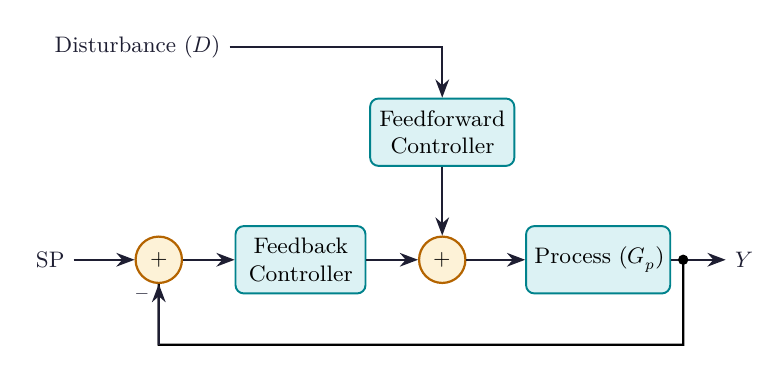
\begin{tikzpicture}[scale=0.9, transform shape]
  \node[sumjunc] (sum1) at (-2.0, 0) {$+$};
  \node[block, text width=1.6cm] (fb) at (0, 0) {Feedback\\Controller};
  \node[sumjunc] (sum2) at (2.0, 0) {$+$};
  \node[block, text width=1.8cm] (proc) at (4.2, 0) {Process ($G_p$)};
  
  \node[block, text width=1.8cm] (ff) at (2.0, 1.8) {Feedforward\\Controller};

  % Paths
  \draw[arrow] (-3.2,0) node[left, font=\small] {SP} -- (sum1);
  \draw[arrow] (sum1) -- (fb);
  \draw[arrow] (fb) -- (sum2);
  \draw[arrow] (sum2) -- (proc);
  \draw[arrow] (proc) -- (6.0, 0) node[right, font=\small] {$Y$};

  % Disturbance feedforward path
  \draw[arrow] (-1.0, 3.0) node[left, font=\small] {Disturbance ($D$)} -- (ff.west |- -1.0, 3.0) -| (ff);
  \draw[arrow] (ff) -- (sum2);
  
  % Feedback loop
  \draw[thick] (5.4, 0) to[short, *-] (5.4, -1.2) -| (sum1);
  \draw[arrow] (-2.0, -1.2) -- (sum1) node[left, pos=0.8, font=\scriptsize] {$-$};
\end{tikzpicture}
\end{tcolorbox}

\begin{itemize}[leftmargin=*, itemsep=2.5pt]
  \item \textbf{Design Equation:} To achieve perfect disturbance cancellation:
    \[
    G_{ff}(s) \cdot G_p(s) + G_d(s) = 0 \Rightarrow G_{ff}(s) = -\frac{G_d(s)}{G_p(s)}
    \]
    where $G_d(s)$ is the disturbance path transfer function and $G_p(s)$ is the process path transfer function.
  \item \textbf{Limitation:} Requires an accurate process model and cannot correct for unmeasured disturbances (hence it is always paired with a feedback controller).
\end{itemize}

\subsection{3. Ratio Control}
Ratio control maintains a fixed ratio between two flows (usually a wild flow $F_w$ and a controlled flow $F_c$, such as fuel-to-air ratio).
\begin{itemize}[leftmargin=*, itemsep=2.5pt]
  \item \textbf{Parallel Configuration:} An operator sets the target total rate; a controller calculates setpoints for both fuel and air flow loops.
  \item \textbf{Series Configuration:} The uncontrolled wild flow is measured, multiplied by a ratio factor $R$, and the result is fed as the setpoint to the controlled flow controller: $SP_c = R \times F_w$.
\end{itemize}

\subsection{4. Split-Range and Override Control}
\begin{itemize}[leftmargin=*, itemsep=2.5pt]
  \item \textbf{Split-Range Control:} A single controller output drives two separate control valves. For example, a $0\text{--}50\%$ output opens a heating steam valve, while $50\text{--}100\%$ opens a cooling water valve.
  \item \textbf{Override (Selective) Control:} Multiple controllers monitor different process variables but output to a single valve. A high/low selector block decides which controller has override authority. Used for limit protection (e.g., maintaining flow rate while overriding to close the valve if pressure exceeds safety limit).
\end{itemize}

\subsection{5. Adaptive Control}
In many industrial processes, the plant dynamics change slowly over time due to wear, temperature drift, aging, or varying operational loads. A standard fixed-parameter PID controller may become unstable or sluggish under these conditions. \textbf{Adaptive control} automatically adjusts the controller parameters online in real-time to maintain desired performance.

\textbf{1. Distinguishing Feature:}
Unlike feedback control (which acts on the error $e(t)$) or feedforward control (which acts on measured disturbances $d(t)$), adaptive control contains a \textbf{parameter adjustment loop} (outer loop) that modifies the controller's gains.

\textbf{2. Core Architectures:}
\begin{itemize}[leftmargin=*, itemsep=2.5pt]
  \item \textbf{Model Reference Adaptive Control (MRAC):}
    \begin{itemize}[leftmargin=*, itemsep=1.5pt]
      \item \textit{Working:} A mathematical \textbf{Reference Model} is chosen to represent the ideal desired closed-loop response. The actual plant output is compared against this reference model output. An adaptation algorithm (e.g., MIT Rule or Lyapunov stability theory) adjusts the controller gains to drive the difference error to zero.
    \end{itemize}
  \item \textbf{Self-Tuning Regulator (STR):}
    \begin{itemize}[leftmargin=*, itemsep=1.5pt]
      \item \textit{Working:} Utilizes a two-step real-time algorithm. First, an online parameter estimator (e.g., Recursive Least Squares --- RLS) identifies the plant's transfer function parameters from input-output data. Second, a controller design block automatically recalculates the controller parameters (e.g., pole placement) based on the newly estimated plant model.
    \end{itemize}
\end{itemize}

\begin{tcolorbox}[tikzbox, title={Model Reference Adaptive Control (MRAC) Architecture}]
\centering
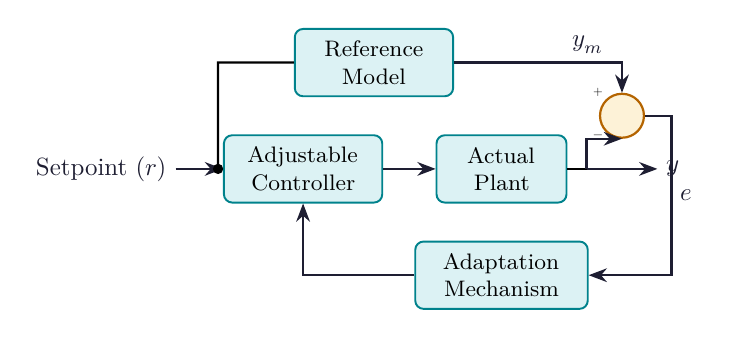
\begin{tikzpicture}[scale=0.9, transform shape]
  % Blocks
  \node[block, text width=2.0cm] (refmodel) at (1.0, 1.5) {Reference\\Model};
  \node[block, text width=2.0cm] (controller) at (0, 0) {Adjustable\\Controller};
  \node[block, text width=1.6cm] (plant) at (2.8, 0) {Actual\\Plant};
  \node[sumjunc] (sum) at (4.5, 0.75) {};
  \node[block, text width=2.2cm] (adapt) at (2.8, -1.5) {Adaptation\\Mechanism};

  % Sign labels on summing junction using anchors to prevent overlaps
  \node[above left, font=\tiny, inner sep=1pt] at (sum.135) {$+$};
  \node[below left, font=\tiny, inner sep=1pt] at (sum.225) {$-$};

  % Paths
  \draw[arrow] (-1.8, 0) node[left] {Setpoint ($r$)} -- (controller);
  \draw[thick] (-1.2, 0) to[short, *-] (-1.2, 1.5) -- (refmodel);
  \draw[arrow] (controller) -- (plant);
  \draw[thick] (plant) -- (4.0, 0);
  \draw[arrow] (4.0, 0) -- (5.0, 0) node[right] {$y$};
  \draw[arrow] (4.0, 0) |- (sum.south);
  \draw[arrow] (refmodel) -| (sum.north) node[above, pos=0.4] {$y_m$};
  \draw[arrow] (sum) -- ++(0.7, 0) |- (adapt) node[right, pos=0.25] {$e$};
  \draw[arrow] (adapt) -| (controller);
\end{tikzpicture}
\end{tcolorbox}

\subsection{6. Internal Model Control (IMC)}
IMC integrates a mathematical model of the process in parallel with the actual plant to predict and reject disturbances.

\begin{tcolorbox}[tikzbox, title={Internal Model Control (IMC) Block Diagram}]
\centering
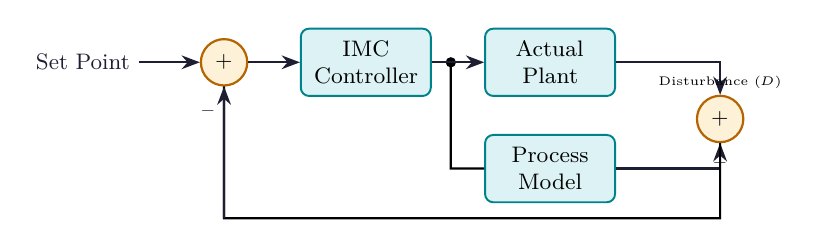
\begin{tikzpicture}[scale=0.9, transform shape]
  \node[sumjunc] (sum1) at (-2.0, 0) {$+$};
  \node[block, text width=1.6cm] (imc) at (0, 0) {IMC\\Controller};
  \node[block, text width=1.6cm] (plant) at (2.6, 0) {Actual\\Plant};
  \node[block, text width=1.6cm] (model) at (2.6, -1.5) {Process\\Model};
  \node[sumjunc] (sum2) at (5.0, -0.8) {$+$};

  % Paths
  \draw[arrow] (-3.2, 0) node[left, font=\small] {Set Point} -- (sum1);
  \draw[arrow] (sum1) -- (imc);
  \draw[thick] (1.2, 0) to[short, *-] (1.2, -1.5) -- (model);
  \draw[arrow] (imc) -- (plant);
  \draw[arrow] (plant) -| (sum2);
  \draw[arrow] (model) -| (sum2) node[below, pos=0.8, font=\scriptsize] {$-$};
  
  \draw[thick] (sum2) -- (5.0, -2.2) -| (sum1);
  \draw[arrow] (-2.0, -2.2) -- (sum1) node[left, pos=0.8, font=\scriptsize] {$-$};
  \node[above, font=\tiny] at (5.0, -0.5) {Disturbance ($D$)};
\end{tikzpicture}
\end{tcolorbox}

\textbf{IMC Controller Design:} If the plant model is $G_m(s)$, the controller is designed as $q(s) = G_m^{-1}(s) \cdot f(s)$, where $f(s)$ is a low-pass filter to guarantee causality and robustness.

\newpage

% ===============================================================================
% QUICK REVISION PAGE
% ===============================================================================
\begin{center}
  {\large\bfseries\color{myred} Quick Revision --- Module 5}\\[3pt]
  {\small\color{mydark} DCS, SCADA \& Advanced Control $|$ PE-EC802B}
\end{center}
\noindent{\color{myred}\rule{\linewidth}{1.2pt}}
\vspace{4pt}

\begin{tcolorbox}[defbox, title={\textbf{One-Line Definitions}}]
\begin{itemize}[leftmargin=*, itemsep=2pt, topsep=0pt]
  \item \textbf{DCS:} A process-oriented control network with distributed processing nodes that handle control loops locally.
  \item \textbf{SCADA:} A geographically wide data acquisition and supervisory system used for utility telemetry and remote control.
  \item \textbf{RTU:} A remote site microprocessor unit that converts field device inputs into telemetry data for SCADA.
  \item \textbf{Feedforward Control:} Open-loop compensation that measures disturbances and takes immediate counter-action.
  \item \textbf{Cascade Control:} A control strategy utilizing nested feedback loops to isolate and reject inner-loop disturbances.
  \item \textbf{Ratio Control:} Control loop configuration maintaining a constant flow ratio between two process streams.
  \item \textbf{Split-Range Control:} Dividing a single controller output range to operate multiple control actuators.
  \item \textbf{Adaptive Control:} A control scheme that automatically adjusts controller parameters in real-time to adapt to changing plant dynamics.
  \item \textbf{Report-by-Exception:} A SCADA communication scheme where remote nodes only transmit data if a value changes beyond a preset limit.
\end{itemize}
\end{tcolorbox}

\begin{tcolorbox}[tikzbox, title={\textbf{Industrial Control Strategy Comparisons}}]
\centering
\par\noindent
\renewcommand{\arraystretch}{1.3}
\begin{tabularx}{\linewidth}{|B{3.0cm}|Y|Y|}
\hline
\textbf{Property} & \textbf{Distributed Control System (DCS)} & \textbf{SCADA System} \\ \hline
\textbf{Syllabus Focus} & Process-oriented (fast loop control, DCS controllers) & Data-oriented (telemetry, remote monitoring) \\ \hline
\textbf{Distribution} & Locally distributed within a plant site & Geographically distributed over wide areas \\ \hline
\textbf{Communication} & Fast, deterministic networks (Ethernet/control rings) & Slow, non-deterministic links (radio, GSM, satellite) \\ \hline
\textbf{Closed-loop Control} & Executes direct loops at controller level & Executes supervisory control (manual/slow setpoint tuning) \\ \hline
\end{tabularx}

\vspace{0.3cm}
\begin{tabularx}{\linewidth}{|B{3.0cm}|Y|Y|}
\hline
\textbf{Property} & \textbf{Feedback Control} & \textbf{Feedforward Control} \\ \hline
\textbf{Control Action} & Corrective (acts *after* output deviates) & Preventive (acts *before* disturbance affects plant) \\ \hline
\textbf{Stability Risk} & High (gain can drive phase delay oscillations) & None (does not introduce feedback poles) \\ \hline
\textbf{Model Requirement} & No model needed (easy PID tuning) & Requires high-accuracy process model ($G_d/G_p$) \\ \hline
\end{tabularx}
\end{tcolorbox}

\begin{tcolorbox}[exambox, title={\textbf{Frequently Asked / Viva Questions}}]
\begin{enumerate}[leftmargin=*, itemsep=4pt]
  \item \Q{Compare DCS and SCADA in terms of architecture and applications.}
    DCS is process-oriented, localized (within a single facility like a chemical plant), and executes fast, closed-loop control over high-bandwidth networks. SCADA is data-oriented, geographically distributed (over thousands of kilometers like a power grid), and relies on low-bandwidth telemetry (radio, GSM) for supervisor-level monitoring and slow-loop adjustments.
  \item \Q{How does Cascade Control improve disturbance rejection?}
    In cascade control, the secondary inner loop operates much faster than the primary outer loop. If a disturbance enters the secondary loop (e.g. feed pressure drops), the secondary controller corrects it immediately before the disturbance can propagate and affect the primary process output.
  \item \Q{Derive the transfer function of an ideal feedforward controller.}
    Let $Y = G_p U + G_d D$ be the process output, where $U$ is control input, $D$ is disturbance, and $G_p, G_d$ are transfer functions. In feedforward control, $U = G_{ff} D$. Substituting $U$ gives $Y = (G_p G_{ff} + G_d) D$. For perfect disturbance cancellation, we require $Y=0$ for any $D \Rightarrow G_p G_{ff} + G_d = 0 \Rightarrow G_{ff}(s) = -G_d(s)/G_p(s)$.
  \item \Q{What is ratio control, and where is it used?}
    Ratio control is an advanced control strategy that maintains a constant ratio between two variable flows (usually fuel and air, or two blending chemicals). It measures a "wild" uncontrolled flow and adjusts a "controlled" flow to match the predefined ratio, preventing incomplete combustion or mixing errors.
  \item \Q{Explain the concept of Split-Range Control with an example.}
    Split-range control splits the output range of a single controller to command multiple actuators. For example, in a reactor temperature loop, a $0\text{--}100\%$ controller output is split: $0\text{--}50\%$ operates a steam valve (for heating), and $50\text{--}100\%$ operates a cooling water valve (for cooling).
  \item \Q{What is Internal Model Control (IMC), and what is its main advantage?}
    IMC is a control structure where a mathematical model of the process is run in parallel with the actual plant. The difference between the plant and model outputs is fed back as an estimate of the net disturbance. This structure simplifies controller design, allows direct control of delays, and guarantees robustness.
  \item \Q{Explain the difference between Model Reference Adaptive Control (MRAC) and Self-Tuning Regulator (STR).}
    MRAC compares the plant's output against the output of a predefined reference model and uses the difference (error) to adjust the controller parameters. STR uses an online parameter estimator (like recursive least squares) to identify the plant parameters in real-time, then recalculates the controller parameters based on the estimated model.
  \item \Q{What is Report-by-Exception (RBE) in SCADA, and why is it used?}
    RBE is an event-driven telemetry scheme where remote terminal units (RTUs) only transmit data to the master terminal unit (MTU) if a variable deviates beyond a preset deadband or if an alarm occurs. It is used to conserve network bandwidth over slow, costly, or congested communication links (like radio or satellite).
\end{enumerate}
\end{tcolorbox}

\end{document}
